% -*- TeX-master: "ijcai18.tex" -*-

\section*{Introduction}\label{sec:intro}

% Introduction rule-based Why uncovering pathways is important What's
% wrong with previous techniques and how they work Overview of the
% solution in a few sentences State contributions precisely Outline of
% the article

Rule-based modeling languages for molecular biology, such as Kappa
\cite{DanosEtAl-CONCUR07} and BioNetGen \cite{bngl}, or organic
chemistry, such as M{\o}d \cite{moll}, can be used to write
mechanistic models of complex reaction systems. In these approaches,
chemical transformations are represented by local graph-rewrite rules
equipped with stochastic firing rates. In a dynamical simulation,
rules induce a time series of events that might reach a state of
interest in processes like the assembly of a molecular machine, the
activation of a transcription factor, or the synthesis of a specific
chemical compound. While rule-based models provide compactness,
transparency, and the ability of handling combinatorial complexity,
the perhaps most significant advantage lies in their suitability for
causal analysis.

% Add a picture of a large story ? - Takes to much space...
% \begin{figure}[!h]
  \vskip -0.1cm
  \begin{center}
    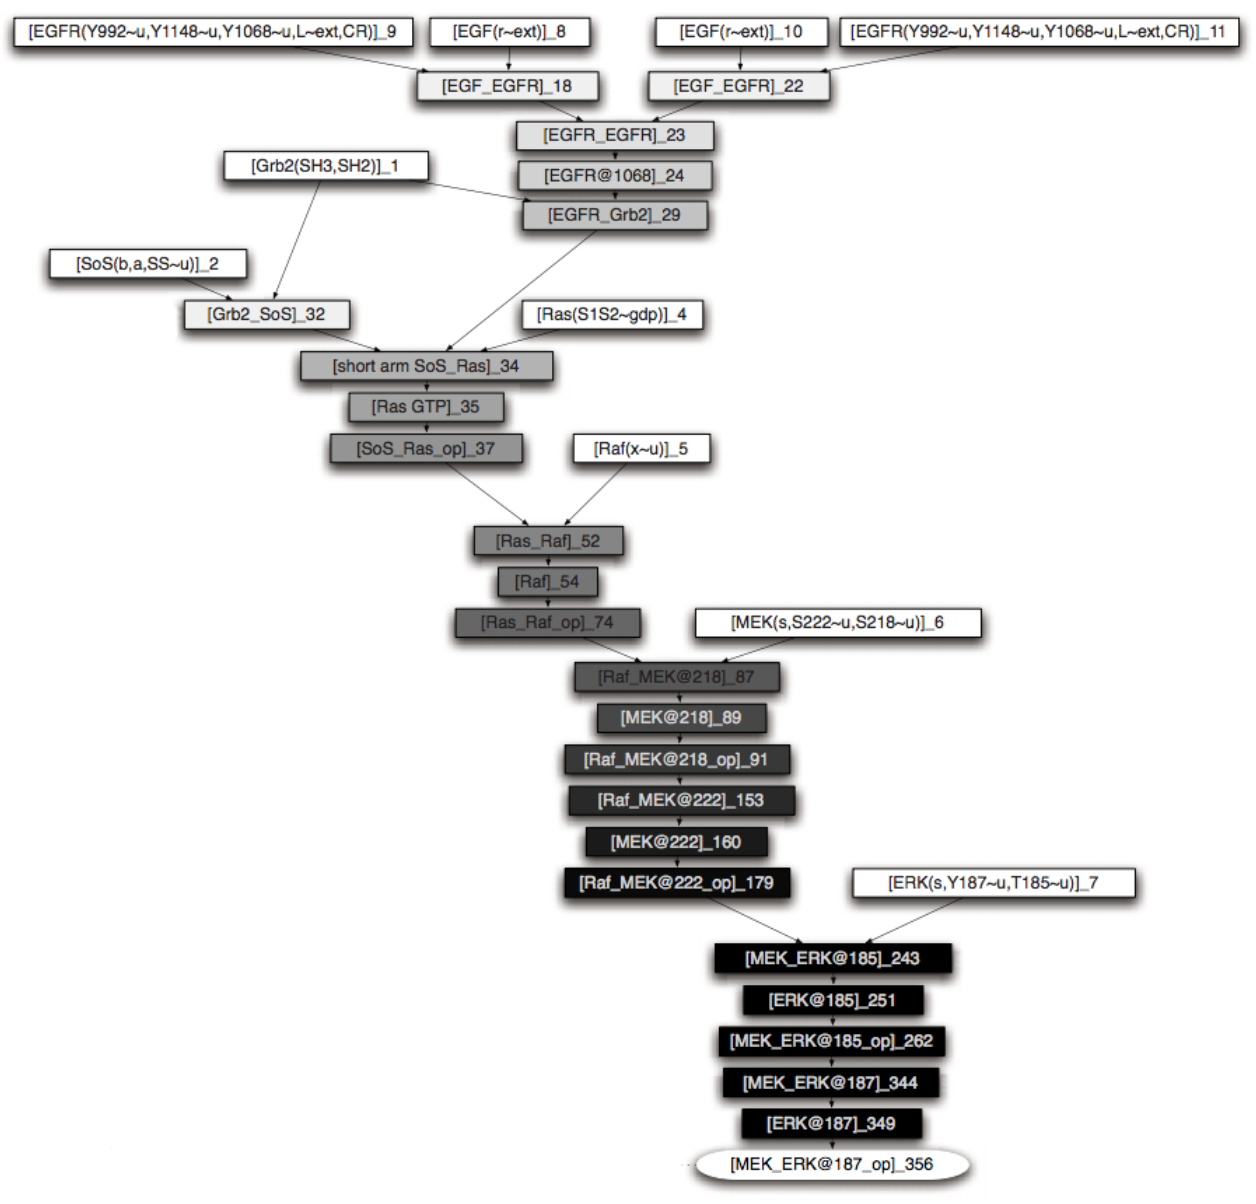
\includegraphics[scale=0.35]{figures/story-egfr.png}
  \end{center}
  \vskip -0.1cm
  \caption{An example of a story describing a part of the EGFR
    signalling pathway, adapted from
    \protect\cite{DanosEtAl-CONCUR07}. Rectangles correspond to
    individual events and solid arrows denote activation between
    them. }
  \label{fig:story-egfr}
\end{figure}


The causal analysis
\cite{DBLP:conf/fsttcs/DanosFFHH12,DanosEtAl-CONCUR07} of event series
generated by such models provides a formal definition of ``pathway"
and a means for revealing the emergence of pathways from low-level
interactions. These methods take advantage of rule structure to
\begin{inparaenum}[(i)]
\item \label{step:compress} compress a given simulation trace into a
  minimal subset of events that are necessary and jointly sufficient
  to replicate a phenomenon of interest and
\item \label{step:highlight} highlight causal influences between
  remaining events, exposing the extent of concurrency.
\end{inparaenum}
Such methods suffer from two major issues though. 

First, step (\ref{step:compress}) as currently implemented is blind to
the kinetics aspect of a model (i.e. the stochastic rates of its
rules).  As a consequence, compressed simulation traces may fail to
include important simulation events that dramatically increase the
probability of observing the phenomenon of interest, although not
structurally necessary in achieving it. Second, step
(\ref{step:highlight}) is limited to a very narrow notion of causal
influence that we call \emph{activation}. Put simply, an event is said
to activate another one if it modifies an aspect of the world that
directly enables the latter to happen. Unfortunately, activation alone
fails at capturing a wide range of causal influences that are
ubiquituous in biology, especially when \emph{inhibition} between
molecular events is at play.  Indeed, an event $a$ may cause an event
$b$ without being transitively activated by it, by preventing an event
$c$ from happening that, had it happened, would have averted
$b$. Uncovering such a causal narrative is challenging because it
involves events that may never be seen during simulation ($c$ in our
example).

In response to those issues, we propose a complementary approach to
causal analysis of event series generated from rule-based models,
which rely on {counterfactual reasoning}. In the tradition of Lewis,
Pearl and Halpern, we investigate possible causal influences by
answering questions of the kind: \textit{``would event $b$ have
  happened had event $a$ not happened ?''}
%\cite{lewis1974causation,pearl2009causality,halpern2016actual},
In this spirit, we claim the following contributions.
\begin{enumerate}
\item We give a semantics account of counterfactual statements in the
  context of rule-based models, where the standard definition of
  counterfactuals based on structural equations
  \cite{pearl2009causality} does not apply. 
\item We show how such statements can be evaluated by sampling
  \emph{counterfactual traces}, which represent how an event series
  may have been different had some external intervention happened. We
  introduce an algorithm to explore such scenarios and
  provide an efficient implementation for the Kappa modelling
  language.
\item We show how counterfactual dependencies between events, once
  discovered, can be explained using a combination of activation and
  inhibition arrows. This results in causal diagrams that come closer
  to the biological intuition of a pathway, where inhibition generally
  plays an important role.
\end{enumerate}
